\section{Solid 1 - SRP, ISP og DIP}

\subsection{Fokuspunkter}

\begin{itemize}
	\item Redegør for designprincipperne:
	\begin{itemize}
		\item Single Responsibility Principle (SRP).
		\item Interface Segregation Principle (ISP).
		\item Dependency Inversion Principle (DIP).
	\end{itemize}
	\item Redegør for, hvordan du mener anvendelsen af principperne fremmer godt SW design.
	\item Vis et eksempel på anvendelsen af et eller flere af principperne i SW design.
	\item Redegør for konsekvenserne ved anvendelsen af principperne - har det nogle ulemper?
\end{itemize}


\subsection{Single Responsibility Principle (SRP)}
En klasse skal kun have ét ansvar. Derved undgår vi at skulle \textit{rebuild, retest and redeploy} funktionalitet, som ikke er ændret.\\

''An axis of change is an axis of change, only if changes occur''\\

''Dont apply SRP if there is no symptom''\\

%% side 118 i Agile derp
Modem eksemplet fra hello: skal vi dele den op? Det kommer an på hvordan applikationen ændrer sig. Hvis connectiondelen ændres skal resten af klassen også rekompilere.

\subsubsection{Brud på SRP}
Brud på SRP kan ses på figur~\ref{fig:ISP_bad}~og~\ref{fig:ISP_good} under ISP i section~\ref{sec:isp}. Hvis dette interface har grund til at blive opdelt så er ansvaret muligvis også så anderledes at det burde være i separate klasser.

\subsection{Interface Segregation Principle (ISP)}\label{sec:isp}
\textit{''No client should be forced to depend on methods it doesn't use''}.\\

Når vi har flere klienter som alle bruger samme klasse gennem et interface \textit{IDoThings} som det kan ses på figur~\ref{fig:ISP_bad} vil nogle klienter blive afhængige af metoder som de ikke bruger.

\begin{figure}[H]
	\centering
	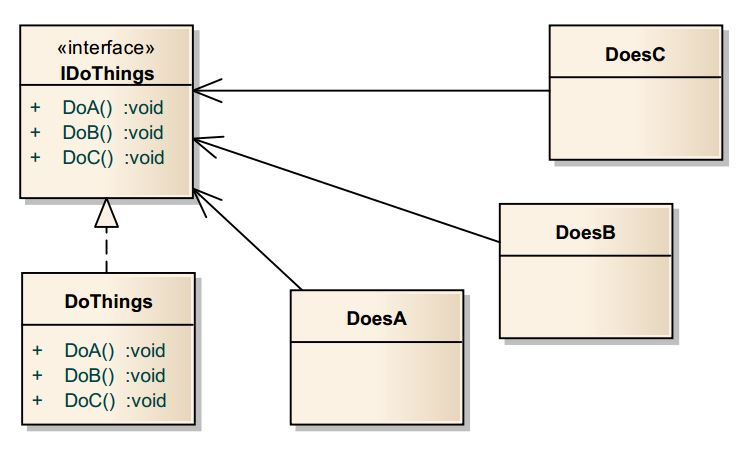
\includegraphics[width=0.7\linewidth]{figs/ISP/ISP_bad}
	\caption{Flere klienter afhængige af samme ''store'' interface.}
	\label{fig:ISP_bad}
\end{figure}

Derfor kan vi ved hjælp af ISP princippet dele interfacet op i flere mindre interfaces. Således undgår vi store og uoverskuelige interfaces, et eksempel er på figur~\ref{fig:ISP_good}.

\begin{figure}[H]
	\centering
	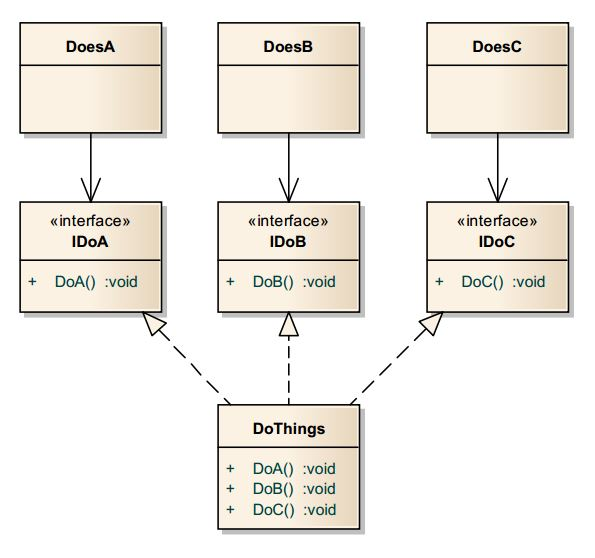
\includegraphics[width=0.7\linewidth]{figs/ISP/ISP_good}
	\caption{ISP anvendt på eksempel fra figur~\ref{fig:ISP_bad}.}
	\label{fig:ISP_good}
\end{figure}

Et eksempel kan være \href{http://code.tutsplus.com/tutorials/solid-part-3-liskov-substitution-interface-segregation-principles--net-36710}{rectangle eksemplet på denne side}. Klassen bør ikke indeholde funktion til både draw() og calc(). Dette gør at at fx GUI includen skal bygges samtidig med calc.

\subsection{Dependency Inversion Principle (DIP)}

\subsection{Hvordan fremmes godt SW design?}

\subsection{Eksempel}

\subsection{Redegør for ulemper}